\documentclass[11pt]{article}

\usepackage[parfill]{parskip}
\usepackage{listings}
\usepackage{fancyvrb}
\usepackage{lipsum}
\usepackage{mathtools}
\usepackage{graphicx}

\title{\textbf{Intrusion Detection Using KDD Dataset}}
\author{GROUP 20\\
		Divya Chaganti\\
		Saili Sahasrabuddhe\\
		Ashwin Viswanathan\\
		Vignesh Miriyala\\
		Sanil Sinai Borkar}
\date{\today}

\begin{document}

\maketitle

% ------------------------------------------ Introduction --------------------------------------------
\section{Introduction}
\label{Sec:Introduction}
Our project is to use a data mining approach to develop an intrusion detection system (IDS) using the KDD dataset~\cite{kdddata}.

% ------------------------------------------ Dataset Stats --------------------------------------------
\section{Dataset}
\label{Sec:Dataset}
The KDD dataset~\cite{kdddata} is a simulated dataset that was generated as part of The 1998 DARPA Intrusion Detection Evaluation Program with the objective of surveying and evaluating research in intrusion detection~\cite{kddnames}. Raw TCP dump data for a local-area network (LAN) simulating a typical U.S. Air Force LAN was collected for nine weeks. The LAN was operated as if it were a true Air Force environment, but was peppered with multiple attacks.

The dataset contains normal packets along with attack packets. The attacks that are included in the dataset can be broadly classified into 4 categories~\cite{kddnames}. The types of attacks present in the dataset are included in each category below:
\begin{enumerate}
\item DOS - denial-of-service\\
E.g.: back, land, neptune, pod, smurf, teardrop
\item R2L - unauthorized access from a remote machine\\
E.g.: ipsweep, portsweep, nmap, satan
\item U2R - unauthorized access to local superuser (root) privileges\\\
E.g.: ftp\_write, guess\_passwd, map, ultihop, hf, py, arezclient, arezmaster
\item Probing - surveillance and other probing\\
E.g.: buffer\_overflow, loadmodule, perl, rootkit, 
\end{enumerate}

The dataset contains 42 features out of which 34 are continuous, 7 are nominal, and the last feature field is the class label indicating the nature of the packets - either `normal' or the type of attack, as specified in Table~\ref{Tab:allfeatures}.

\begin{table}
\caption{Dataset Feature Set}
\centering
\begin{tabular}{ll}
Feature & Type \\
\hline
duration & continuous \\
protocol\_type & symbolic \\
service & symbolic \\
flag & symbolic \\
src\_bytes & continuous \\
dst\_bytes & continuous \\
land & symbolic \\
wrong\_fragment & continuous \\
urgent & continuous \\
hot & continuous \\
num\_failed\_logins & continuous \\
logged\_in & symbolic \\
num\_compromised & continuous \\
root\_shell & continuous \\
su\_attempted & continuous \\
num\_root & continuous \\
num\_file\_creations & continuous \\
num\_shells\ & continuous \\
num\_access\_files & continuous \\
num\_outbound\_cmds & continuous \\
is\_host\_login & symbolic \\
is\_guest\_login & symbolic \\
count & continuous \\
srv\_count & continuous \\
serror\_rate & continuous \\
srv\_serror\_rate & continuous \\
rerror\_rate & continuous \\
srv\_rerror\_rate & continuous \\
same\_srv\_rate & continuous \\
diff\_srv\_rate & continuous \\
srv\_diff\_host\_rate & continuous \\
dst\_host\_count & continuous \\
dst\_host\_srv\_count & continuous \\
dst\_host\_same\_srv\_rate & continuous \\
dst\_host\_diff\_srv\_rate & continuous \\
dst\_host\_same\_src\_port\_rate & continuous \\
dst\_host\_srv\_diff\_host\_rate & continuous \\
dst\_host\_serror\_rate & continuous \\
dst\_host\_srv\_serror\_rate & continuous \\
dst\_host\_rerror\_rate & continuous \\
dst\_host\_srv\_rerror\_rate & continuous \\
attack\_type & symbolic \\
\end{tabular}
\label{Tab:allfeatures}
\end{table}

The total number of records for each attack are given in Table~\ref{Tab:numRecs}.
\begin{table}
\caption{Number of records for each attack}
\centering
\begin{tabular}{ll}
Type of attack & Number of records \\
\hline
back & 2203 \\
buffer\_overflow & 30 \\
ftp\_write & 8 \\
guess\_passwd & 53 \\
imap & 12 \\
ipsweep & 1247 \\
land & 21 \\
loadmodule &  9 \\
multihop & 7 \\
neptune &  107201 \\
nmap &  231 \\
normal &  97278 \\
perl &  3 \\
phf &  4 \\
pod &  264 \\
portsweep &  1040 \\
rootkit &  10 \\
satan &  1589 \\
smurf &  280790 \\
spy &  2 \\
teardrop &  0 \\
warezclient &  1020 \\
warezmaster &  20 \\
total & 494021 \\
\end{tabular}
\label{Tab:numRecs}
\end{table}



% ------------------------------------------ Literature Review --------------------------------------------
\section{Literature Review}
\label{Sec:Lit}
Since this is an old dataset, significant research has been done in this area. Kuchimanchi et al.~\cite{DimRed} perform dimensionality reduction using Principal Component Analysis (PCA) and considered 19 principal components using Eigen value decomposition and decreasing standard deviations. We have performed only PCA present in R libraries and selected 11 out of the 42 features.

Some significant research using the KDD dataset is done on anomaly-based and misuse-based detection techniques~\cite{detkdd}. By statistically analyzing the entire KDD data set, the analysis showed that there are two important issues in the data set which highly affects the performance of evaluated systems and results in a very
poor evaluation of anomaly detection approaches. A new data set NSL-KDD is proposed, which consists of selective records of the complete KDD data set as a solution to the said problem.

We have used decision trees in our project to classify and predict the results while this project uses different methods like Na{\"i}ve Bayes. Also, Weka's default values are as the input parameters of these methods.

Machine learning algorithms also have been applied to the KDD 1999 Cup intrusion detection dataset resulted in dismal performance for user-to-root and remote-to-local attack categories~\cite{sabhnani2003application}. Nine distinct pattern recognition and machine learning algorithms were tested on the KDD dataset. These algorithms were selected so that they represent a wide variety of fields: neural networks, probabilistic models, statistical models, fuzzy-neuro systems, and decision trees.

In our project, we predict whether the given request is an attack or legitimate request. In contrast to this, the authors have tried to identify whether it belongs to any particular attack category like user-to-root etc.


% ------------------------------------------ Feature Extraction --------------------------------------------
\section{Feature Extraction}
\label{Sec:Feature}
The original KDD dataset contains 42 features including the label. Since working this size of data may not be feasible always from the perspective of a real-time IDS, we had to reduce the number of features used. This was achieved by using PCA. 34 of the 42 features of the dataset were continuous on which PCA was applied.

Out of all the 34 continuous features, we picked up the principal components that contained positive weights for most of the {\it error rate} indicating features. Out of the 34 candidate principal components, we narrowed down it to 2 principal components, and selected the one that had more positive weights. This led us to finalize our principal component which is specified below:

$Comp 23 = 0.124*num\_access\_files - 0.131*serror\_rate + 0.141*srv\_serror\_rate - 0.490*srv\_rerror\_rate + 0.107*same\_srv\_rate + 0.126*diff\_srv\_rate - 0.154*dst\_host\_diff\_srv\_rate + \\ 0.263*dst\_host\_srv\_diff\_host\_rate - 0.122*dst\_host\_serror\_rate + 0.162*dst\_host\_srv\_serror\_rate + 0.717*dst\_host\_rerror\_rate$

Based on this principal component, 11 features were selected out of the available 41 as shown in Table~\ref{Tab:features} as per the description given in \cite{kddnames}.

\textbf{Note: PCA was used only to give us an insight on the variations that are exhibited by the various features and to determine which features account for what percentage of the entire dataset. The `Comp23' contains a linear combination of features which accounts for a major portion of the dataset. Hence, these only these features were considered. All the algorithms were not run on the principal components, but on the original data containing only the said features.}

\begin{table}
\caption{Final Feature Set}
\centering
\begin{tabular}{l*{2}{l}}
Feature & Description \\
\hline
num\_access\_files & number of operations on access control files  \\
serror\_rate & \% of connections that have ``SYN'' errors  \\
srv\_serror\_rate & \% of connections that have ``SYN'' errors  \\
srv\_rerror\_rate & \% of connections that have ``REJ'' errors  \\
same\_srv\_rate & \% of connections to the same service \\
diff\_srv\_rate & \% of connections to different services \\
dst\_host\_diff\_srv\_rate &  \\
dst\_host\_srv\_diff\_host\_rate &  \\
dst\_host\_serror\_rate &  \\
dst\_host\_srv\_serror\_rate &  \\
dst\_host\_rerror\_rate &  \\
\end{tabular}
\label{Tab:features}
\end{table}

% ------------------------------------------ Classification --------------------------------------------
\section{Classification}
\label{Sec:Class}
\subsection{Methods and Materials}

\subsubsection{Package Used}
{\it J48} - RWeka~\cite{rweka}

\subsubsection{Feature Selection}

We tried running classification on the entire dataset but obtained the following results:
\begin{enumerate}
\item Classification
\begin{itemize}
\item Accuracy: 76.87\%
\item Time Taken: 36 seconds
\end{itemize}
\item Prediction
\begin{itemize}
\item Accuracy: 76.28\%
\item Time Taken: 0.5 seconds
\end{itemize}
\end{enumerate}

Although this is not a very bad degree of accuracy, it is unacceptable for an IDS. Moreover, the prediction time is a bit on the higher side. Hence, the 11 features obtained by using PCA in Section~\ref{Sec:Feature} was used.

\subsubsection{Classifier}
Decision Tree classifier was used to classify the instances. Out of the 494022 packets, 80\% of it was used as training data (395218 records), and the remaining 20\% was used for testing (98803 records).

Since the IDS needs to tag each network packet as either malicious (attack packet) or benign (normal packet), the type of attack is not significant but only the presence of an attack packet is. Therefore, as a pre-processing step for classification, the normal packets were labeled as `normal' and everything else was tagged as an `attack' packet.

\subsection{Results}
\subsubsection{Training}

The time taken to train a decision tree classifier model was around {\bf 14 seconds} on an average, and accuracy was {\bf 95.5318\%}. The summary of the classifier model is given below:

\begin{Verbatim}[fontsize=\small]
=== Summary ===

Correctly Classified Instances      377559               95.5318 %
Incorrectly Classified Instances     17659                4.4682 %
Kappa statistic                          0.8471
Mean absolute error                      0.083 
Root mean squared error                  0.2037
Relative absolute error                 26.2432 %
Root relative squared error             51.2282 %
Coverage of cases (0.95 level)          99.8133 %
Mean rel. region size (0.95 level)      81.0894 %
Total Number of Instances           395218     

=== Confusion Matrix ===

      a      b   <-- classified as
 316384   1011 |      a = attack.
  16648  61175 |      b = normal.
\end{Verbatim}

\subsubsection{Prediction}
The prediction for the 98803 records was done in {\bf 0.2 seconds} with an accuracy of {\bf 95.46\%}. The confusion matrix for the prediction is given below:

\begin{Verbatim}[fontsize=\small]
Confusion Matrix and Statistics

          Reference
Prediction attack. normal.
   attack.   79084    4223
   normal.     264   15232
                                          
               Accuracy : 0.9546          
                 95% CI : (0.9533, 0.9559)
    No Information Rate : 0.8031          
    P-Value [Acc > NIR] : < 2.2e-16       
                                          
                  Kappa : 0.8445          
 Mcnemar's Test P-Value : < 2.2e-16       
                                          
            Sensitivity : 0.9967          
            Specificity : 0.7829          
         Pos Pred Value : 0.9493          
         Neg Pred Value : 0.9830          
             Prevalence : 0.8031          
         Detection Rate : 0.8004          
   Detection Prevalence : 0.8432          
      Balanced Accuracy : 0.8898          
                                          
       'Positive' Class : attack.  
\end{Verbatim}      

% ------------------------------------------ Association --------------------------------------------
\section{Association}
\label{Sec:Assoc}

\subsection{Methods and Materials}
Our dataset contains packet information for 24 attack types. The goal of the association analysis task was to find out relevant rules for each attack with the attack type in the RHS. In other words, rules stating the presence of certain values for different packet fields which lead to different attacks.

\subsubsection{Packages Used}
arules~\cite{arules}, arulesViz~\cite{arulesViz}, Matrix~\cite{matrix}

\subsubsection{Feature Selection}
There are 43 features in the dataset out of which 34 attributes were used based on domain knowledge and results of PCA. 

\subsubsection{Data preparation}
Since only 7 out of the selected 34 attributes were discrete, remaining 27 attributes had to be discretized. We used `discretize' method from the package `arules' and chose the method of discretization for each attribute by looking at the value distribution. As an example, there are 14 attributes which provide the percentage error rate and have values in the range 0 - 1, these were discretized into 10 intervals with fixed interval of 0.1.

\subsubsection{Rule generation}
The support value was chosen based on the number of records for each attack and the total number of attacks in the dataset to ensure that some rules are found and the confidence used was 0.9 and max length of rules was restricted to 5. Also redundant rules were removed to find unique rules for each attack.

\subsection{Results}
Some of the interesting rules found were as follows:

\begin{itemize}
\item If the packet is for `telnet' service on the destination, root shell is obtained and the number of connections to same service on destination is between 90 to 100 percent, then the attack is buffer overflow.
\item The presence of urgent indicator in packet and targeted towards `login' service on destination and number of operations on access control files equal to 1 indicate a ftp\_write attack.
\item If number of failed login attempts is greater than zero and flag is set to reset connection then the attack is guess password.
\item If the packet is targeted for `imap' service on the destination and the number of connections to same service on destination is between 90 to 100 percent, then the attack is imap.
\item If the number of connections to different hosts is between 40-50\% and the packet is for `eco\_i' service on destination then the attack is ipsweep.
\item If the attribute land is 1 i.e. if connection is from/to the same host/port then the attack is land.
\item If the number of shell prompts obtained is 2 and number of operations on access control files equal to 1 then the attack is loadmodule.
\item If the wrong fragment is 1 then attack is ping of death.
\item If the root shell is obtained and the urgent indicator is 1 then the attack is rootkit.
\end{itemize}

\begin{Verbatim}[fontsize=\tiny]
#  Back attack

lhs                          rhs                support     confidence lift    
1 {hot=2}                   => {attack_type=back} 0.004305485 0.9703467  217.5995
2 {num_compromised=[1,884]} => {attack_type=back} 0.004309533 0.9572842  214.6702

#  Buffer overflow

lhs                                     rhs                                support confidence     lift
1  {service=telnet,                                                                                      
    root_shell=1,                                                                                        
    num_shells=0,                                                                                        
    dst_host_same_srv_rate=[0.9,1.0]}   => {attack_type=buffer_overflow} 3.238729e-05  1.0000000 16467.37
2  {service=telnet,                                                                                      
    num_compromised=[1,884],                                                                             
    num_shells=0,                                                                                        
    dst_host_same_srv_rate=[0.9,1.0]}   => {attack_type=buffer_overflow} 3.643570e-05  0.9473684 15600.66
3  {service=telnet,                                                                                      
    root_shell=1,                                                                                        
    num_root=0}                         => {attack_type=buffer_overflow} 3.238729e-05  0.9411765 15498.70

# ftp_write

 lhs                                                 rhs                     support      confidence lift    
1  {urgent=2}                                       => {attack_type=ftp_write} 2.024205e-06 1          61752.62
2  {service=login,urgent=2}                         => {attack_type=ftp_write} 2.024205e-06 1          61752.62
3  {urgent=2,num_access_files=1}                    => {attack_type=ftp_write} 2.024205e-06 1          61752.62

# guess_password

lhs                                        rhs                             support confidence     lift
1  {hot=1,                                                                                               
    num_failed_logins=1}                   => {attack_type=guess_passwd} 9.513766e-05  1.0000000 9321.151
2  {flag=RSTO,                                                                                           
    num_failed_logins=1}                   => {attack_type=guess_passwd} 9.108925e-05  1.0000000 9321.151
3  {num_failed_logins=1,                                                                                 
    dst_host_rerror_rate=[0.9,1.0]}        => {attack_type=guess_passwd} 8.299242e-05  1.0000000 9321.151
	
# imap

lhs                                                 rhs                support      confidence lift    
1 {service=imap4,dst_host_same_srv_rate=[0.9,1.0]} => {attack_type=imap} 2.226626e-05 1          41168.42
2 {service=imap4,flag=SF}                          => {attack_type=imap} 1.214523e-05 1          41168.42
3 {service=imap4,same_srv_rate=[0.9,1.0]}          => {attack_type=imap} 2.429047e-05 1          41168.42

# ipsweep

lhs                                        rhs                       support confidence     lift
1 {service=eco_i,                                                                                 
   dst_host_srv_diff_host_rate=[0.4,0.5)} => {attack_type=ipsweep} 0.001333951  0.9939668 393.7775
2 {srv_diff_host_rate=[0.9,1.0],                                                                  
   dst_host_srv_diff_host_rate=[0.4,0.5)} => {attack_type=ipsweep} 0.001311685  0.9863014 390.7406
3 {wrong_fragment=0,                                                                              
   dst_host_same_src_port_rate=[0.9,1.0],                                                         
   dst_host_srv_diff_host_rate=[0.4,0.5)} => {attack_type=ipsweep} 0.001333951  0.9441261 374.0322
   
# land
 
  lhs         rhs                support      confidence lift   
1 {land=1} => {attack_type=land} 4.250831e-05 0.9545455  22455.5


# loadmodule

lhs                                        rhs                           support confidence     lift
1 {num_shells=2,                                                                                      
   dst_host_srv_rerror_rate=[0.1,0.2)}    => {attack_type=loadmodule} 2.024205e-06          1 54891.22
2 {num_shells=2,                                                                                      
   num_access_files=1}                    => {attack_type=loadmodule} 2.024205e-06          1 54891.22
3 {num_shells=2,                                                                                      
   dst_host_srv_diff_host_rate=[0.2,0.3)} => {attack_type=loadmodule} 2.024205e-06          1 54891.22



# multihop

lhs                                        rhs                         support confidence     lift
1 {hot=15}                                => {attack_type=multihop} 2.024205e-06          1 70574.43
2 {hot=3,                                                                                           
   num_shells=2}                          => {attack_type=multihop} 2.024205e-06          1 70574.43
3 {num_shells=1,                                                                                    
   num_access_files=2}                    => {attack_type=multihop} 2.024205e-06          1 70574.43

# neptune

lhs                                   rhs                   support   confidence lift    
44 {protocol_type=tcp,logged_in=0}    => {attack_type=neptune} 0.2169968 0.9175968  4.228618
1  {service=private}                  => {attack_type=neptune} 0.2050864 0.9136465  4.210414
2  {dst_host_same_srv_rate=[0.0,0.1)} => {attack_type=neptune} 0.2143350 0.9081677  4.185166

# nmap

 lhs                                        rhs                     support confidence     lift
1 {flag=SH}                               => {attack_type=nmap} 0.0002084932  0.9626168 2058.671
2 {service=eco_i,                                                                               
   srv_diff_host_rate=[0.9,1.0],                                                                
   dst_host_srv_diff_host_rate=[0.2,0.3)} => {attack_type=nmap} 0.0002003963  0.9339623 1997.389
3 {protocol_type=icmp,                                                                          
   srv_diff_host_rate=[0.9,1.0],                                                                
   dst_host_srv_diff_host_rate=[0.2,0.3)} => {attack_type=nmap} 0.0002003963  0.9339623 1997.389
   
# perl

lhs                                        rhs                     support confidence     lift
1 {num_shells=1,                                                                                
   dst_host_rerror_rate=[0.6,0.7)}        => {attack_type=perl} 2.024205e-06          1 164673.7
2 {root_shell=1,                                                                                
   dst_host_rerror_rate=[0.6,0.7)}        => {attack_type=perl} 2.024205e-06          1 164673.7
3 {num_file_creations=[1,28],                                                                   
   dst_host_rerror_rate=[0.6,0.7)}        => {attack_type=perl} 2.024205e-06          1 164673.7
   
# phf
 
 lhs                                        rhs                    support confidence     lift
1 {root_shell=1,                                                                               
   srv_rerror_rate=[0.5,0.6)}             => {attack_type=phf} 2.024205e-06          1 123505.2
2 {root_shell=1,                                                                               
   srv_diff_host_rate=[0.9,1.0]}          => {attack_type=phf} 2.024205e-06          1 123505.2
3 {service=http,                                                                               
   root_shell=1,                                                                               
   num_access_files=1}                    => {attack_type=phf} 8.096822e-06          1 123505.2
   
# pod

lhs                   rhs               support      confidence lift   
1 {wrong_fragment=1} => {attack_type=pod} 0.0005242692 0.9664179  1808.45

# portsweep

lhs                                        rhs                         support confidence     lift
1 {dst_host_diff_srv_rate=[0.9,1.0],                                                                
   dst_host_same_src_port_rate=[0.9,1.0],                                                           
   dst_host_rerror_rate=[0.9,1.0]}        => {attack_type=portsweep} 0.001024248          1 475.0202
2 {dst_host_diff_srv_rate=[0.9,1.0],                                                                
   dst_host_same_src_port_rate=[0.9,1.0],                                                           
   dst_host_srv_rerror_rate=[0.9,1.0]}    => {attack_type=portsweep} 0.001014127          1 475.0202
3 {rerror_rate=[0.9,1.0],                                                                           
   dst_host_diff_srv_rate=[0.9,1.0],                                                                
   dst_host_same_src_port_rate=[0.9,1.0]} => {attack_type=portsweep} 0.001014127          1 475.0202
   
# rootkit

lhs                                     rhs                   support      confidence lift   
1 {urgent=1,root_shell=1}              => {attack_type=rootkit} 2.024205e-06 1          49402.1
2 {urgent=1,hot=1}                     => {attack_type=rootkit} 2.024205e-06 1          49402.1
3 {urgent=1,num_file_creations=[1,28]} => {attack_type=rootkit} 2.024205e-06 1          49402.1


# satan

lhs                                        rhs                     support confidence     lift
1 {same_srv_rate=[0.0,0.1),                                                                     
   diff_srv_rate=[0.9,1.0]}               => {attack_type=satan} 0.002841984  1.0000000 310.9006
2 {flag=REJ,                                                                                    
   diff_srv_rate=[0.9,1.0],                                                                     
   dst_host_same_src_port_rate=[0.0,0.1)} => {attack_type=satan} 0.002487748  0.9967559 309.8920
3 {diff_srv_rate=[0.9,1.0],                                                                     
   dst_host_same_src_port_rate=[0.0,0.1),                                                       
   dst_host_srv_rerror_rate=[0.9,1.0]}    => {attack_type=satan} 0.002487748  0.9959481 309.6408
   
 # smurf
 
 lhs                                        rhs                   support confidence     lift
1 {service=ecr_i}                         => {attack_type=smurf} 0.5683766  0.9978323 1.755583
2 {protocol_type=icmp}                    => {attack_type=smurf} 0.5683766  0.9900847 1.741952
3 {dst_host_same_src_port_rate=[0.9,1.0]} => {attack_type=smurf} 0.5680508  0.9636522 1.695446
 
 # spy

 lhs                                     rhs                    support confidence     lift
1 {su_attempted=1,                                                                          
   num_shells=1}                       => {attack_type=spy} 2.024205e-06          1 247010.5
2 {su_attempted=1,                                                                          
   dst_host_serror_rate=[0.2,0.3)}     => {attack_type=spy} 2.024205e-06          1 247010.5
3 {su_attempted=1,                                                                          
   num_access_files=1}                 => {attack_type=spy} 2.024205e-06          1 247010.5
 
# warezclient
 
 lhs                                        rhs                           support confidence     lift
1 {service=ftp_data,                                                                                  
   logged_in=1,                                                                                       
   dst_host_same_src_port_rate=[0.9,1.0]} => {attack_type=warezclient} 0.001307637  0.9124294 441.9209
2 {service=ftp_data,                                                                                  
   logged_in=1,                                                                                       
   dst_host_same_srv_rate=[0.9,1.0]}      => {attack_type=warezclient} 0.001283346  0.9109195 441.1896
 
# warezmaster
 
 lhs                                                  rhs                       support      confidence lift    
1 {hot=18,num_file_creations=[1,28]}                => {attack_type=warezmaster} 2.024205e-06 1          24701.05
2 {hot=18,dst_host_same_srv_rate=[0.0,0.1)}         => {attack_type=warezmaster} 2.024205e-06 1          24701.05
3 {is_guest_login=1,dst_host_serror_rate=[0.3,0.4)} => {attack_type=warezmaster} 2.024205e-06 1          24701.05
\end{Verbatim}


% ------------------------------------------ Clustering --------------------------------------------
\section{Clustering}
\label{Sec:Clust}

\subsection{Methods and Materials}
\subsubsection{Packages Used}
{\it kmeans} - stats~\cite{stats}, {\it preprocess} - caret~\cite{caret}, {\it predict} - caret, {\it plot} - 3d~\cite{3d}

\subsubsection{Approaches}
Using k-means clustering to do clustering.We observed that most of the fields describing the data are continuous and hence we thought using a distance based approach is a good idea.
We are not using any features which has factor data as we are using distance based clustering

\subsubsection{Feature Selection - All Features vs PCA}
Initially we have tried to take all the components but the ratio was pretty low ($between\_SS / total\_SS$).
Of the continuous variables on our dataset we have done PCA and generated all the principal components and then we switched to taking only the principal components generated after doing PCA and we have observed that the ratio improved drastically after that.

\subsubsection{Data Preparation - Scaling and Center}
We found that each of the dimensions have different range like {\it src\_bytes}, {\it dest\_bytes} and {\it num\_of\_files} each have different range. So we have done scaling and centering so that clustering is not biased on one particular feature.We have also observed that improved the results.

\subsubsection{Sampling of Different Attacks}
We have also observed that our dataset has more points for two particular types of attacks and few points for one of the attack and hence we thought equal sampling of the data would be a good thing to do but turns out that it did not really affect the result, the accuracy did not improve.

\subsection{Results}

The dataset contains 23 different types of attacks which are further divided to into 5 broad classes. So we have tried to different total cluster sizes i.e. 23 and 5 and results turned out to be good in case of 23 classes as compared to 5 which kind of makes sense because though the class of attacks belong to the same broad category but are very spread out in the feature space and this will affect clustering adversely.

\subsubsection{Number of classes - 5}

Within cluster sum of squares by cluster:

[1]  24304.94  56739.37 112714.73 147962.42 803257.83

$ (between\_SS / total\_SS =  78.9 \%)$

The plot for clustering on 5 attack classes is given in Figure~\ref{clust5}.

\begin{figure}[htp]
\centering
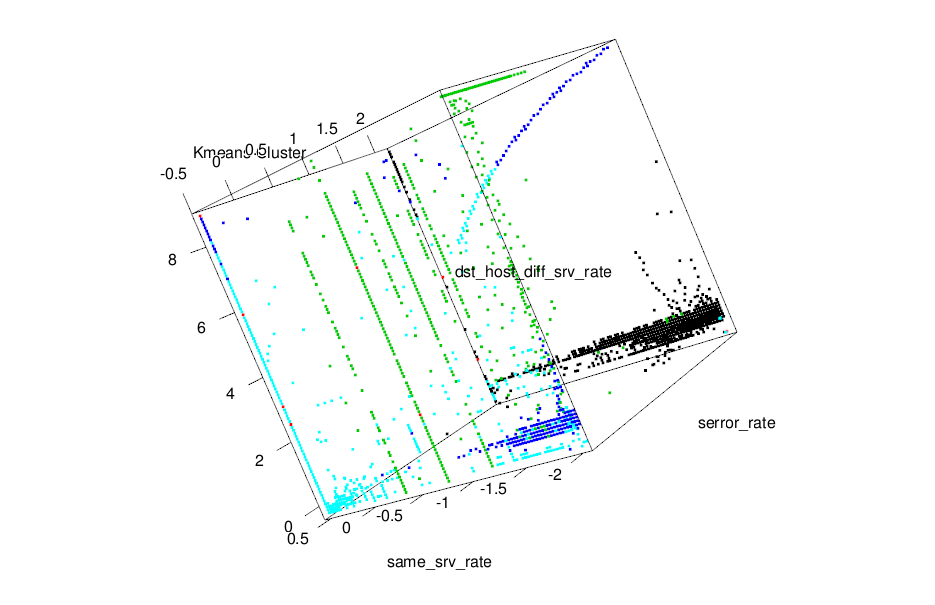
\includegraphics[scale=0.40]{images/clust-5.png}
\caption{Clustering Results for 5 attack classes}
\label{clust5}
\end{figure}

\subsubsection{Number of classes - 23}

Within cluster sum of squares by cluster:

[1]  3227.35686  1272.85737  1961.66395   710.47783  4834.37121   411.49075  2932.80823 47009.93535 42451.05736
 
[10]   667.83164    98.60543  3878.55384 26582.85832  1080.77894  1747.93551  1604.59234  3298.17346  3274.04034

[19]  7064.86597  6587.84850 85157.18493  1487.41422  1936.37399

$ (between\_SS / total\_SS =  95.4\%)$

The plot for clustering on all 23 attack classes is given in Figure~\ref{clust23}.

\begin{figure}[htp]
\centering
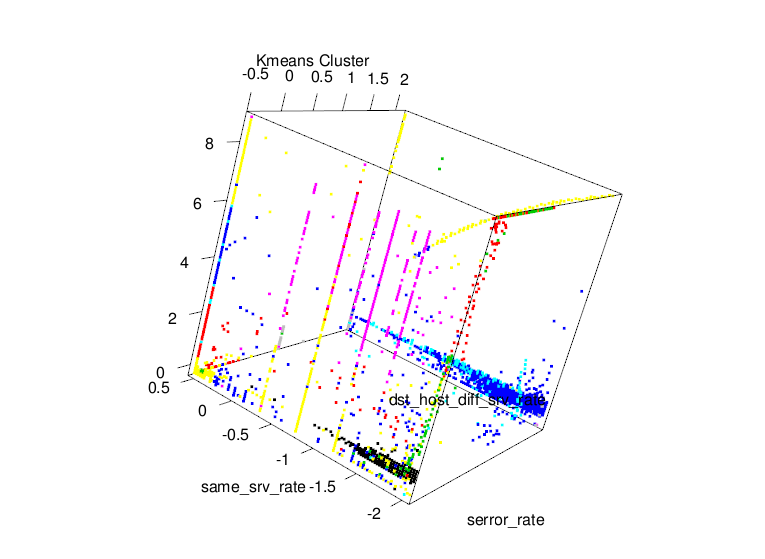
\includegraphics[scale=0.40]{images/clust-23.png}
\caption{Clustering Results for 23 attack classes}
\label{clust23}
\end{figure}


% ------------------------------------------ Discussion --------------------------------------------
\section{Discussion}
\label{Sec:Disc}

\subsection{Classification}
Since we are designing a real-time IDS, we were more interested in an approach that performs prediction very fast. For the said reason, \textbf{decision tree (C4.5)} was used as a classifier as it learned the trained data with an accuracy of \textbf{95.53\%} in \textbf{14 seconds} on an average for nearly \textbf{400K data packets}. This large learning time is acceptable as training the classifier is a periodic activity (maybe once a day). Decision tree classifier also predicts in a very short time, as we required. It predicted around \textbf{98K data packets} with an accuracy of \textbf{95.46\%} in just \textbf{0.2 seconds}.

\subsection{Association}
Majority of the data features are continuous, so we performed discretization on these features based on the spread of values in each feature. Association analysis was carried out by using the \textbf{apriori} method. The final rules obtained by eliminating redundant rules. The rules for many attacks found by association analysis are found to be in sync with domain knowledge expectations. We used varying values of support for different types based on the number of records for each attack. Confidence value of {\bf 0.9} was chosen to remove possibility of any false positives.

\subsection{Clustering}
Since majority of the features are continuous, it was reasonable to use a distance-based clustering method like \textbf{kMeans}. Some of the attributes had different ranges, we used scaling and centering which actually improved our results. We carried kMeans to find 2 different sets of clusters - one with 5 classes (which included normal data and the broad classes mentioned in Section \ref{Sec:Dataset}), and one with 23 classes (which included normal data and all the types of attacks mentioned in the examples in Section \ref{Sec:Dataset}).

% ------------------------------------------ Conclusion --------------------------------------------
\section{Conclusion}
\label{Sec:Concl}

Since we dealt with a large number of features, we had to use a dimensionality reduction technique. PCA was found to be the easiest and most effective method for dimensionality reduction as it reduced the number of features from 42 to just 11. We even tried with the original dataset without using PCA, and found unimpressive and erroneous results. It was necessary to discretize the continuous features in order to find useful rules which would not have been generated without the use of these continuous features. Moreover, the data contained a lot of features which had varying ranges. Thus, for a distance-based clustering method, it was necessary to scale such data to obtain unbiased clustering. We tried clustering on raw data to find unimpressive results.

For much better results, it would have been useful if we could generate new genuine http data to predict. However, the dataset is an old simulated dataset and most of the fields that it contains are not present in the TCP headers that are currently used today. Therefore, this seems an impossible task to achieve.

% ------------------------------------------ References --------------------------------------------
\bibliographystyle{IEEEtran}
\bibliography{Reference}

\end{document}